%% LyX 2.0.6 created this file. For more info, see http://www.lyx.org/.
%% Do not edit unless you really know what you are doing.
\documentclass[twocolumn,prl,aps,twocolumn]{revtex4-1}
\setcounter{secnumdepth}{3}
\usepackage{amsmath}
\usepackage{amssymb}
\usepackage{graphicx}
\usepackage{esint}
\usepackage[unicode=true,pdfusetitle,
 bookmarks=false,
 breaklinks=false,pdfborder={0 0 1},backref=false,colorlinks=false]
 {hyperref}
\hypersetup{
 bookmarksnumbered=false,bookmarksopen=false}

\makeatletter
%%%%%%%%%%%%%%%%%%%%%%%%%%%%%% Textclass specific LaTeX commands.
\@ifundefined{textcolor}{}
{%
 \definecolor{BLACK}{gray}{0}
 \definecolor{WHITE}{gray}{1}
 \definecolor{RED}{rgb}{1,0,0}
 \definecolor{GREEN}{rgb}{0,1,0}
 \definecolor{BLUE}{rgb}{0,0,1}
 \definecolor{CYAN}{cmyk}{1,0,0,0}
 \definecolor{MAGENTA}{cmyk}{0,1,0,0}
 \definecolor{YELLOW}{cmyk}{0,0,1,0}
}

%%%%%%%%%%%%%%%%%%%%%%%%%%%%%% User specified LaTeX commands.
\usepackage{color}
\usepackage{soul}
\newcommand{\note}[1]{\textcolor{blue}{(#1)}}
\newcommand{\MP}[1]{\textcolor{magenta}{#1}}
\newcommand{\wzy}[1]{\textcolor{red}{#1}}

\newcommand{\CNV}{$^{13}$C }


\makeatother

\begin{document}

\title{Controlling Spectrally-indistinguishable Nuclear Spins \\ for a
  Decoherence-Free Subspace}


\author{Michael A. Perlin}
\affiliation{Institut f\"ur Theoretische Physik and IQST, Albert-Einstein-Allee
11, Universit\"at Ulm, D-89069 Ulm, Germany}

\author{Zhen-Yu Wang}
\email{zhenyu3cn@gmail.com}
\affiliation{Institut f\"ur Theoretische Physik and IQST, Albert-Einstein-Allee
11, Universit\"at Ulm, D-89069 Ulm, Germany}

\author{Jorge Casanova}
\affiliation{Institut f\"ur Theoretische Physik and IQST, Albert-Einstein-Allee
11, Universit\"at Ulm, D-89069 Ulm, Germany}

\author{Martin. B. Plenio}
\affiliation{Institut f\"ur Theoretische Physik and IQST, Albert-Einstein-Allee
11, Universit\"at Ulm, D-89069 Ulm, Germany}


\begin{abstract}
  Close nuclear spins with identical precession frequencies have the
  remarkable property of feeling the same magnetic noise, which makes
  them exceptional candidates for constructing a decoherence-free
  subspace (DFS). However, selective control of such nuclei is not
  possible with existing methods based on spectroscopic
  discrimination. We overcome this obstacle and present a protocol for
  storage and retrieval of quantum information from a DFS. We
  demonstrate the efficacy of our protocol with detailed numerical
  simulations of a nitrogen-vacancy (NV) center with nearby \CNV
  nuclei, and show that the resulting DFS is immune to NV magnetic
  noise and external magnetic field drifts.
\end{abstract}
\maketitle

\emph{Introduction.}~-- Quantum spins in a solid-state platform are
natural and reliable quantum resources for performing tasks such as
information processing, simulations, and nano-scale
sensing~\cite{Zhong2015Optically, Doherty2013Nitrogen,
  Dobrovitski2013Quantum, Schirhagl2014Nitrogen}. A particularly
promising platform containing such resources is the nitrogen-vacancy
(NV) center in diamond~\cite{Doherty2013Nitrogen,
  Dobrovitski2013Quantum, Schirhagl2014Nitrogen}. \MP{At room
  temperature, the electron spin of an NV center has a $T_1$-limited
  lifetime on the order of milliseconds, as $T_2$ decoherence
  processes can be suppressed via dynamical decoupling
  techniques~\cite{Jarmola12, vanderSar12}. During this time, the
  electron spin can be polarized, detected, and coherently manipulated
  with high fidelity via optical fields and microwave
  radiation~\cite{Taminiau14}. By working at lower temperatures and
  high purity diamond samples, the electron spin lifetime can be
  extended upwards to seconds~\cite{Gill13}.}
% old text here: At room temperature, the electron spins of NV centers
% have coherence times on the order of milliseconds, and can be
% polarized, detected, and coherently manipulated with high fidelity
% via optical fields and microwave radiation~\cite{Jarmola12,
% vanderSar12, Taminiau14}. By working at lower temperatures and
% employing dynamical decoupling techniques, these coherence times can
% be extended upwards to seconds~\cite{Gill13}.
Furthermore, the NV electron spin can be selectively coupled to nearby
\CNV nuclear spins by appropriately controlling individual
electron-nuclear hyperfine interactions. In this manner, nuclear spins
can be individually addressed and manipulated via the NV center when
they have distinct precession frequencies $\omega_{j}$, with $j$
indexing a particular nucleus. These distinctions are a consequence of
the energy shifts produced by the components $A_{j}^{\parallel}$ of
the hyperfine field parallel to the NV symmetry axis at the location
of the each nucleus~\cite{Kolkowitz2012Sensing,Taminiau2012Detection,
  Zhao2012Sensing}. Individual addressing allows for the realization
of noise-resilient quantum gates~\cite{Liu2013Noise}, quantum error
correcting codes~\cite{Taminiau2014Universal, Waldherr2014Quantum},
quantum computing~\cite{Casanova2016Noise}, and quantum simulation
protocols~\cite{Cai2013Large} in the hybrid system of a NV center and
its surrounding nuclei. In addition, the NV electron spin provides an
optical interface to entangle spins with
photons~\cite{Togan2010Quantum}, which together with the available
nuclear memory establishes a key prerequisite for scalable quantum
architectures~\cite{Nemoto2014Photonic}. To this end, recent
remarkable experiments have established photon-mediated entanglement
between distant NV quantum-network
nodes~\cite{Bernien2013Entanglement,
  Pfaff2014Unconditional,Hensen2015Loophole}, as well as entanglement
distillation on entangled spin qubits~\cite{Kalb2016Entanglement}.

% todo: insert citations 24, 31, and 32 into first paragraph

\begin{figure}[t!]
  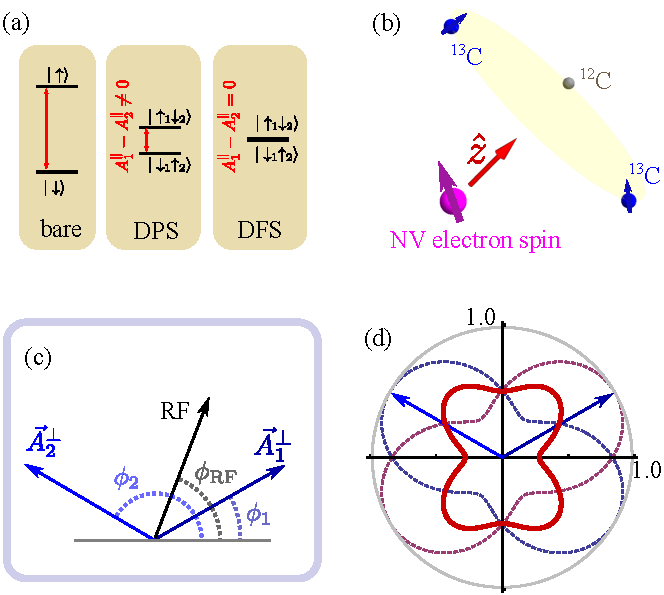
\includegraphics[width=0.95\columnwidth]{FigDrawing}
  \caption{(Color online) (a) Energy splittings of bare, DPS, and DFS
    qubit states. (b) A pair of \CNV nuclear spins located in a
    symmetric configuration about the NV center have the same parallel
    and perpendicular components of the hyperfine field. (c)
    Perpendicular hyperfine components of the spin pair in (b) and the
    effective direction of a RF field. (d) Polar plot of the NV
    transition signal (red solid line) with respect to the RF phase
    $\phi_{{\rm RF}}$. Dashed lines show the polar plots of single
    spin signals, and the gray solid circle is the single spin signal
    without RF control.}
\label{fig:Drawing}
\end{figure}

Although strong electron-nuclear hyperfine interactions are generally
desirable for fast and reliable nuclear spin control via the NV
center, these strong interactions can also dephase the nuclear
spins~\cite{Maurer2012Room} % removed citation for Wang2017Delayed
due to, for example, electron spin relaxation. More specifically, the
electron undergoes stochastic spin flips ($T_1$ processes), thereby
acting as a source of magnetic noise for the nuclear spins. This noise
is most severe during the optical initialization and readout of NV
electrons, as well as during the reset for establishing
electron-photon entanglement~\cite{Reiserer2016Robust}\MP{, and cannot
  be suppressed with dynamical decoupling techniques}.
% Because these NV electron spin flips are much faster than external
% radio frequency control over nuclei, noise suppression techniques
% such as dynamical decoupling~\cite{Yang2011Preserving} are incapable
% of prolonging nuclear spin coherence times.
Electron spin noise thus limits the use of individual nuclear spins as
a quantum resource. While nuclear spins with weaker hyperfine coupling
to the NV center are less sensitive to electron spin flip noise, weak
coupling also unavoidably implies poor nuclear spin controllability,
which again limits their utility for quantum memory registers.

By pairing nuclear spins, one can reduce the magnitude of NV electron
spin noise on individual qubits by constructing decoherence-protected
subspaces (DPS)~\cite{Reiserer2016Robust} {[}see
Fig.~\ref{fig:Drawing}(a){]}.  Similar to standard techniques in
nuclear magnetic resonance (NMR)~\cite{Mehring1983Principle} or
electron-nuclear double resonance
(ENDOR)~\cite{Schweiger2001Principles}, current protocols for
realizing a DPS rely on the distinct nuclear precession frequencies
$\omega_{j}$ for addressing and control~\cite{Kolkowitz2012Sensing,
  Taminiau2012Detection, Zhao2012Sensing, Liu2013Noise,
  London2013Detecting, Taminiau2014Universal, Casanova2015Robust,
  Wang2016Positioning, Wang2017Delayed}. The logical qubits in a DPS
are therefore still sensitive to electron spin
noise~\cite{Reiserer2016Robust}.

In this work, we address the problem of selectively manipulating
nuclear spins with identical precession frequencies $\omega_{j}$ by
combining dynamical decoupling techniques with radio-frequency (RF)
nuclear spin control. As a result, we are able to construct an
accessible decoherence-free subspace (DFS) in a solid-state platform,
and thereby realize robust quantum memory registers which are
resilient to dephasing processes such as NV initialisation and
readout. Among the possible applications of this work, we highlight
storage of the electron spin state into the DFS, leaving the NV center
free to perform other tasks such as forming entangled quantum
networks.

\emph{Electron-nuclear coupling.}~-- In the typical situation with the
electron-nuclear flip-flop terms suppressed by a large energy
mismatch, on the order of GHz in the case of an NV center and nearby
\CNV nuclei, the hyperfine interactions between the electron and
nuclear spins reads
$H_{{\rm hf}}=S_{z}\sum_{j}\vec{A}_{j}\cdot\vec{I}_{j}$, where $S_{z}$
and $\vec{I}_{j}$ are respectively electron and nuclear spin
operators. Denoting by $\hat{z}$ a unit vector along the NV symmetry
axis, the hyperfine fields $\vec{A}_{j}$ can be decomposed into
parallel and perpendicular components
$A_{j}^{\parallel}=\vec{A}_{j}\cdot\hat{z}$ and
$\vec{A}_{j}^{\perp}=\vec{A}_{j}-A_{j}^{\parallel}\hat{z}$. In the
presence of a static magnetic field $B_{z}\hat{z}$ with strength
$B_z\gg A_{j}^{\perp}/\gamma_{\rm n}$, where $\gamma_{\rm n}$ is the
nuclear \CNV gyromagnetic ratio, the perpendicular components
$\vec{A}_{j}^{\perp}\cdot\vec{I}_{j}=A_{j}^{\perp}I_{j}^{x}$ in
$H_{{\rm hf}}$ are suppressed, resulting in the coupling (see for
example~\cite{Maurer2012Room})
\begin{equation}
  H_{{\rm hf}} = S_{z}\sum_{j}A_{j}^{\parallel}I_{j}^{z},
  \label{eq:SzIz}
\end{equation}
where $I_{j}^{z}=\vec{I}_{j}\cdot\hat{z}$. While nuclear spins are
excellent candidates for a quantum memory, uncontrolled electron spin
flips generate random noise with the strengths $A_{j}^{\parallel}$ on
the nuclei through the coupling in Eq.~\eqref{eq:SzIz}.

By pairing nuclear spins, the strength of dephasing noise can be
diminished to $\delta_{1,2}=A_{1}^{\parallel}-A_{2}^{\parallel}$ in a
DPS~\cite{Reiserer2016Robust}. Existing protocols for selective spin
manipulation, however, have gate times on the scale of
$1/\delta_{1,2}$, which are furthermore bounded from above by the NV
electron spin coherence time. This restriction is prohibitive for the
realization of an accessible DFS, which requires $\delta_{1,2}=0$
{[}see Fig.~\ref{fig:Drawing}(a){]}.

\emph{Larmor pairs.}~-- Due to symmetries of the diamond lattice, it
is possible for multiple \CNV nuclear spins to share the same
hyperfine components $A_{j}^{\parallel}=A^{\parallel}$ and
$A_{j}^{\perp}=A^{\perp}$. Such nuclei manifestly satisfy the
necessary conditions for containing a DFS. We refer to exactly two
\CNV nuclei in such a symmetric configuration {[}see
Fig.~\ref{fig:Drawing}(b){]} as a \emph{Larmor pair}, and observe
their relatively large probability of occurrence in an NV system with
natural \CNV abundance {[}see Fig.~\ref{fig:FigChance}{]}. Because
$A^{\parallel}$ for the Larmor pair is different from the parallel
hyperfine field $A_{j}^{\parallel}$ of other spins, we can use our
recently developed dynamical decoupling
sequence~\cite{Casanova2015Robust} to selectively couple the NV
electron to only the Larmor pair, realizing the effective interaction
Hamiltonian
\begin{equation}
  H_{{\rm int}}
  = \frac{1}{4}f_{k_{{\rm DD}}}A^{\perp}\sigma_{z}(I_{1}^{x}+I_{2}^{x}),
  \label{eq:Hint}
\end{equation}
where $f_{k_{{\rm DD}}}$ is a tunable parameter of the dynamical
decoupling sequence~\cite{Casanova2015Robust} and $\sigma_{z}$ is an
electron spin Pauli operator. The Hamiltonian in Eq.~\eqref{eq:Hint}
generates the entangling gate
\begin{equation}
  U_{{\rm int}}(\theta)
  = \exp\left[-i\theta\sigma_{z}(I_{1}^{x}+I_{2}^{x})\right]
  \label{eq:Uint}
\end{equation}
with an interaction time $4\theta/(f_{k_{{\rm DD}}}A^{\perp})$.

To find a Larmor pair, we use the recently developed delayed
entanglement echo (DEE) in \cite{Wang2017Delayed} to find spectrally
resolvable resonances, and identify the number of nuclear spins within
them. Having found a Larmor pair, we can measure the corresponding
hyperfine fields $\vec{A}_{j}^{\perp}$ via our recently developed
nuclear positioning method in \cite{Wang2016Positioning}. Therein, we
turn on an external RF magnetic field on resonance with the nuclear
spin precession frequency. In the rotating frame of the nuclear spin
precession, the phase of this RF field corresponds to an effective
static magnetic field direction $\phi_{\rm{RF}}$ in the $x$-$y$ plane
{[}see Fig.~ \ref{fig:Drawing}(c) and (d){]}. When the effective field
direction is parallel to $\vec{A}_{j}^{\perp}$, the electron-nuclear
spin coupling vanishes for spin $j$; an effective field direction not
parallel to $\vec{A}_{j}^{\perp}$ will simply reduce the magnitude of
this coupling. By varying the phase of the RF field, one can thus
measure the positions of both nuclei in the Larmor pair. This
measurement can be simplified by taking symmetries of the diamond
lattice into account {[}see Fig.~\ref{fig:Drawing}(d) for the NV
transition signal in a strong magnetic field{]}. The ambiguity of
$180^{\circ}$ in Fig.~\ref{fig:Drawing}(d) can be eliminated by
checking the NV transition signal in the presence of a weak magnetic
field ($B_{z}\sim A_{j}^{\perp}/\gamma_{{\rm n}}$)
\cite{Wang2016Positioning}. As we will see, however, resolving this
ambiguity is not necessary for our protocol.

\begin{figure}[t!]
  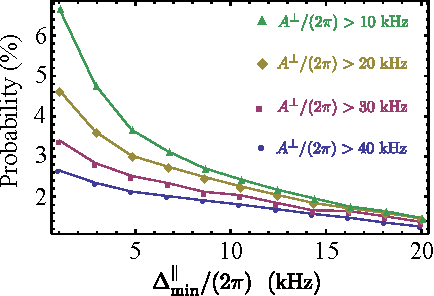
\includegraphics[width=0.95\columnwidth]{FigChance}
  \caption{(Color online) Probability to find at least one Larmor pair
    near the NV electron spin for a natural \CNV abundance of
    1.1\%. Different markers denote different minimum values of the
    $A^\perp$, which couples the nuclei to the NV electron spin, and
    $\Delta_{{\rm min}}^{\parallel}$ is the minimum difference between
    $A^\parallel$ and the parallel hyperfine field for any other \CNV
    nucleus in the NV system. Each of spin in the Larmor pair is
    coupled to other nuclear spins with a strength smaller than
    $2\pi\times50$ Hz, and the directions of hyperfine fields satisfy
    the constrain Eq.~\eqref{eq:AngleRange}.  Each data point is
    obtained via Monte Carlo sampling with $4\times10^{5}$ randomly
    generated NV systems.}
\label{fig:FigChance}
\end{figure}

\emph{Controlling spectrally indistinguishable nuclear spins}. -- The
symmetry between nuclear spins in Eq.~\eqref{eq:Hint} can be broken by
a RF control field, allowing for individual control of each nucleus in
a Larmor pair. Using the technique outlined in
\cite{Wang2016Positioning}, we can decouple all electron-nuclear
interactions, and introduce RF control fields targeting the desired
Larmor pair in a coherence-protected manner to realize the Hamiltonian
\begin{equation}
  H_{{\rm RF}}
  = \vec{\Omega}(\phi_{{\rm RF}})\cdot(\vec{I}_{1}+\vec{I}_{2})
  = \Omega(I_{1}^{\phi_{{\rm RF}}-\phi_{1}}+I_{2}^{\phi_{{\rm RF}}-\phi_{2}}),
  \label{eq:Hrf}
\end{equation}
where $\phi_{j}$ are the azimuthal angles of the perpendicular
components of the local hyperfine fields {[}see Fig.~\ref{fig:Drawing}
(c){]}; $I_{j}^{\phi}=I_{j}^{x}\cos\phi+I_{j}^{y}\sin\phi$; and
$\Omega$, $\phi_{{\rm RF}}$ are respectively the Rabi frequency and
phase of the RF drive. Note that the spin operators $I_{j}^{x}$ are
quantized along the azimuthal directions of their respective local
hyperfine fields $\vec{A}_{j}^{\perp}$. By combining the non-selective
control of $H_{{\rm RF}}$ and $H_{{\rm int}}$, we can selectively
address only one of the two nuclei in the Larmor pair. Without loss of
the generality, we let the index $j=1$ for the target nucleus.

The control in Eq.~\eqref{eq:Hrf} allows us to apply $\pi$ pulses on
both nuclei simultaneously by applying the RF drive for a time
$\pi/\Omega$. Using $\phi_{{\rm RF}}=\phi_{2}+\pi/2$ and defining
$\alpha=\phi_{2}-\phi_{1}+\frac{\pi}{2}$, we can thus generate the
gate
\begin{equation}
  U_{\pi} = \exp(i\pi I_{2}^{y})\exp(i\pi I_{1}^{\alpha}).
  \label{eq:Upi}
\end{equation}
One can then show that the sequence
\begin{equation}
  U_{{\rm DEE}}
  = U_{{\rm int}}(\theta)U_{\pi}U_{{\rm int}}(\theta)
\end{equation}
leads to the evolution $U_{{\rm DEE}}=\exp(i\pi I_{2}^{y})U_{1}$,
where
\begin{equation}
  U_{1} = e^{-i\theta\sigma_{z}I_{1}^{x}}e^{i\pi I_{1}^{\alpha}}
  e^{-i\theta\sigma_{z}I_{1}^{x}}
\end{equation}
entangles only the target nucleus with the NV electron. We can cancel
the single-qubit operation on the second spin by repeating the
sequence $U_{{\rm DEE}}$ twice to get
\begin{eqnarray}
  U_{{\rm DEE}}^{2}
  & = & -2i(r_{x}I_{1}^{\alpha}+r_{y}I_{1}^{\alpha_{\perp}})\sigma_{z}
        \nonumber \\
  &  & +\cos^{2}\theta-\cos(2\alpha)\sin^{2}\theta,
       \label{eq:Udee}
\end{eqnarray}
where we define
$r_{x}=2\cos\alpha\sin\theta
\left[\cos^{2}\alpha\cos\theta+\sin^{2}\alpha\right]$;
$r_{y}=4\cos^{2}\alpha\sin\alpha\sin\theta\sin^{2}(\frac{\theta}{2})$;
and $\alpha_{\perp}=\alpha+\pi/2$. The last line of
Eq.~\eqref{eq:Udee} vanishes when
\begin{equation}
  \cos^{2}\alpha\sin^{2}\theta=\frac{1}{2},
  \label{eq:PiPulseCondition}
\end{equation}
which can be satisfied by choosing a suitable value of $\theta$ if
\begin{equation}
  \left|\sin(\phi_{2}-\phi_{1})\right|\ge1/\sqrt{2}.
  \label{eq:AngleRange}
\end{equation}
While we will work within the constraint of Eq.~\eqref{eq:AngleRange},
we note that it is possible to relax this constraint by applying
additional repetitions of $U_{{\rm DEE}}$. By using a value of
$\theta$ which satisfies Eq.~\eqref{eq:PiPulseCondition}, we can
implement a selective $\pi$ rotation $R_{\pi}$ on the target spin
along a direction perpendicular to $\hat{z}$ by applying
$U_{{\rm DEE}}^2$ followed by a $\sigma_z$ gate on the electron spin,
i.e.
\begin{equation}
  R_{\pi} = \sigma_{z}U_{{\rm DEE}}^{2} = \exp(-i\pi I_{1}^{\beta}),
  \label{eq:PiPulse}
\end{equation}
where the azimuthal angle $\beta$ can be determined from
Eqs.~\eqref{eq:Udee} and \eqref{eq:PiPulseCondition}. From
Eq.~\eqref{eq:Udee} and the definition of $\alpha$, we can see that
the ambiguity of $\pi$ in $\phi_{1}$ and $\phi_{2}$
[Fig.~\ref{fig:Drawing}(d)] is inconsequential as it merely introduces
a possible global phase in the nuclear spin gate
Eq.~\eqref{eq:PiPulse}. Using Eq.~\eqref{eq:PiPulse}, we can implement
a selective controlled phase gate on only one spin in a Larmor pair,
such as
\begin{equation}
  U_{{\rm ent}}
  = (i\sigma_{x}R_{\pi}e^{-iH_{{\rm hf}}\tau})^{2}
  = \exp(-2i\tau A_{1}^{\parallel}I_{1}^{z}),
\end{equation}
which borrows the idea from DEE of having two blocks of control-free
evolution $e^{-iH_{{\rm hf}}\tau}$ driven by Eq.~\eqref{eq:SzIz}.

\begin{figure}[t!]
  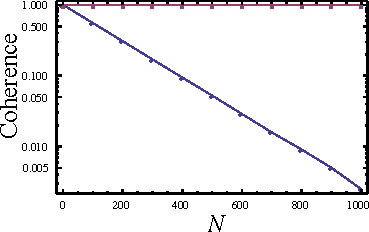
\includegraphics[width=0.95\columnwidth]{FigCoherence}
  \caption{(Color online) Coherence of the Larmor pair, initialized in
    the superposition state
    $(1/\sqrt{2})\left(|\uparrow_{1}\downarrow_{2}\rangle
      +|\downarrow_{1}\uparrow_{2}\rangle\right)$, as a function of
    optical illumination periods ($N$). In each $10~\mu$s period, we
    apply a $\pi$ pulse on the electron spin to simulate gate
    operations on the electron spin, which can affect the
    electron-nuclear spin dynamics. Blue spheres are the case of a DPS
    with $\omega_{1}-\omega_{2}=2\pi\times6.7$ kHz, while red squares
    are the case of a DFS.}
  \label{fig:FigCoherence}
\end{figure}

We performed numerical simulations to demonstrate the high fidelity of
our selective control in Eq.~\eqref{eq:PiPulse}. In these simulations,
we consider a Larmor pair positioned on a diamond lattice at
$[0.1785,0.1785,1.071]$ nm and $[0.1785,1.071,0.1785]$ nm relative to
the NV defect location, each at a distance of approximately $1.1$ nm
from the NV electron. A magnetic field of $B_{z}=0.4$ T is applied
along the NV axis $\hat{z}=[1,1,1]/\sqrt{3}$. The two nuclear spins
have identical hyperfine components $A^{\parallel}=2\pi\times10.2$ kHz
and $A^{\perp}=2\pi\times22.2$ kHz. to realise the sequence in
Eq.~\eqref{eq:PiPulse}, we use adaptive-XY-8 (AXY-8) sequences working
at the $17$-th harmonic to generate the interaction of
Eq.~\eqref{eq:Hint} in a robust manner. The entire protocol, during
which the electron spin coherence is protected by the AXY-8 sequence,
takes $\approx 504~\mu$s. Our numerical simulations include 1208
microwave $\pi$ pulses, each with a duration of 25 ns, while to meet
with realistic experimental conditions we considered a 1$\%$ amplitude
and $2\pi\times2.162$ MHz detuning errors for these pulses. Under
these conditions, we achieve a fidelity of 0.994.

\emph{Nuclear spin DFS in solids.}~-- Using selective control on each
of the spins in the Larmor pair, we can construct a DFS
$\{|\uparrow_{1}\downarrow_{2}\rangle,
|\downarrow_{1}\uparrow_{2}\rangle\}$ in their joint Hilbert
space. The coherence of the state in the DFS is insensitive to optical
and microwave control on the NV electron spin, yielding much longer
coherence times than the case of a DPS, as shown in
Fig.~\ref{fig:FigCoherence}.

One can initialize the Larmor pair into the state
$|\uparrow_{1}\downarrow_{2}\rangle$ within the DFS by first
polarizing the nuclear spins to $|\downarrow_{1}\downarrow_{2}\rangle$
via either SWAP operations with the NV electron spin or dynamical
nuclear polarization, and then using the nuclear-selective $\pi$
rotation in Eq.~\eqref{eq:PiPulse} to flip the first spin. Below, we
describe protocols for quantum information storage in and retrieval
from the DFS.

\emph{Storing the electron spin state in a DFS}. -- A general quantum
state $c_{0}|0\rangle+c_{1}|1\rangle$ of the electron spin can be
stored in a DFS by the following steps. With the Larmor pair
initialized to $|\uparrow_{1}\downarrow_{2}\rangle$, we apply the
conditional evolution $U_{{\rm int}}(\frac{\pi}{2})$
{[}Eq.~\eqref{eq:Uint}{]} to achieve the entangled electron-nuclear
spin state
$c_{0}|0\rangle|y_{1}^{-}y_{2}^{+}\rangle -
c_{1}|1\rangle|y_{1}^{+}y_{2}^{-}\rangle$, where $|y_{j}^{\pm}\rangle$
denotes $\exp(\pm i\frac{\pi}{2}I_{j}^{x})|\downarrow_{j}\rangle$.
Then we apply a $\pi/2$ pulse on the electron spin followed by a
projective measurement on the NV electron to get
$|0\rangle\left(c_{0}|y_{1}^{-}y_{2}^{+}\rangle +
  c_{1}|y_{1}^{+}y_{2}^{-}\rangle\right)$ or
$|1\rangle\left(c_{0}|y_{1}^{-}y_{2}^{+}\rangle -
  c_{1}|y_{1}^{+}y_{2}^{-}\rangle\right)$. The optical readout
subsequently polarizes the NV to the state
$|0\rangle$~\cite{Reiserer2016Robust}. Finally, we apply the
conditional evolution $U_{{\rm int}}(\frac{\pi}{2})$ to get
$c_{0}|\uparrow_{1}\downarrow_{2}\rangle +
c_{1}|\downarrow_{1}\uparrow_{2}\rangle$ if the previous measurement
outcome was $m_{s}=0$, or
$c_{0}|\uparrow_{1}\downarrow_{2}\rangle -
c_{1}|\downarrow_{1}\uparrow_{2}\rangle$ if it was $m_{s}=1$.

\emph{Retrieval of a quantum state from the DFS}. -- To retrieve the
quantum information stored in the DFS, say,
$c_{0}|\uparrow_{1}\downarrow_{2}\rangle +
c_{1}|\downarrow_{1}\uparrow_{2}\rangle$, we can use the following
steps: (i) We apply a selective $\pi$ rotation via
Eq.~\eqref{eq:PiPulse} to flip the first spin and get
$c_{0}|\uparrow_{1}\uparrow_{2}\rangle +
c_{1}|\downarrow_{1}\downarrow_{2}\rangle$. (ii) We initialize the
electron spin state to the superposition
$|x_{e}^{+}\rangle=\left(|0\rangle+|1\rangle\right)/\sqrt{2}$. (iii)
We apply a standard DEE protocol as in Ref.~\cite{Wang2017Delayed} to
achieve the interaction
$A^{\parallel}\sigma_{z}(I_{1}^{z}+I_{2}^{z})$, which implements a
conditional phase gate on the electron spin and yields
$c_{0}|y_{e}^{+}\rangle|\uparrow_{1}\uparrow_{2}\rangle +
c_{1}|y_{e}^{-}\rangle|\downarrow_{1}\downarrow_{2}\rangle$, where
$|y_{e}^{\pm}\rangle = \exp(\mp
i\frac{\pi}{4}\sigma_{z})|x_{e}^{+}\rangle$. (iv) We apply a $\pi/2$
pulse on the electron spin to get
$c_{0}|0\rangle|\uparrow_{1}\uparrow_{2}\rangle -
c_{1}|1\rangle|\downarrow_{1}\downarrow_{2}\rangle$. (v) Finally, we
use the conditional evolution $U_{{\rm int}}(\frac{\pi}{2})$
{[}Eq.~\eqref{eq:Uint}{]} to retrieve the state as
$\left(c_{0}|0\rangle+c_{1}|1\rangle\right)|x_{1}^{+}x_{2}^{+}\rangle$,
where the nuclear spin states can be reset to the state
$|\uparrow_{1}\downarrow_{2}\rangle$ in the DFS by a $\pi$ pulse as in
Eq.~\eqref{eq:PiPulse}.

\emph{Conclusions}. -- We proposed a scheme to selectively address
nuclear spins that have identical hyperfine field components and
Larmor precession frequencies. By using this scheme, we construct a
decoherence-free subspace of nuclear spin states for reliable quantum
storage in a solid-state platform, even in the presence of the noisy
NV center electron spin dynamics. We provided a protocol to store
quantum states of the NV electron in the DFS, and a complementary
protocol to retrieve a quantum state from the DFS back into the NV
electron spin. Our methods are general and can be applied to other
color centers such as silicon carbide. Our results are useful for
building robust optical interfaces for quantum networks and the
realization of DFS quantum information processing, as well as in
quantum sensing.

\begin{thebibliography}{10}
\bibitem{Zhong2015Optically}M. Zhong, M. P. Hedges, R. L. Ahlefeldt,
J. G. Bartholomew, S. E. Beavan, S. M. Wittig, J. J. Longdell, and
M. J. Sellars, Optically addressable nuclear spins in a solid with
a six-hour coherence time, Nature (London) \textbf{517}, 177 (2015).

\bibitem{Doherty2013Nitrogen}M. W. Doherty, N. B. Manson, Paul Delaney,
F. Jelezko, J. Wrachtrup, and L. C. L. Hollenberg, The nitrogen-vacancy
colour centre in diamond, Phys. Rep. \textbf{528}, 1 (2013).

\bibitem{Dobrovitski2013Quantum}V. V. Dobrovitski, G. D. Fuchs, A.
L. Falk, C. Santori, and D. D. Awschalom, Quantum control over single
spins in diamond, Annu. Rev. Condens. Matter Phys. \textbf{4}, 23
(2013).

\bibitem{Schirhagl2014Nitrogen}R. Schirhagl, K. Chang, M. Loretz,
and C. L. Degen, Nitrogen-vacancy centres in diamond: nanoscale sensors
for physics and biology, Annu. Rev. Phys. Chem. \textbf{65}, 83 (2014).

\bibitem{Jarmola12} A. Jarmola, V. M. Acosta, K. Jensen, S. Chemerisov, and D. Budker, Temperature- and Magnetic-Field-Dependent Longitudinal Spin Relaxation in Nitrogen-Vacancy Ensembles in Diamond, Phys. Rev. Lett. \textbf{108}, 197601 (2012).

\bibitem{vanderSar12} T. van der Sar, Z. H. Wang, M. S. Blok, H. Bernien,	T. H. Taminiau, D. M. Toyli, D. A. Lidar, D. D. Awschalom, R. Hanson, and V. V. Dobrovitski, Decoherence-protected quantum gates for a hybrid solid-state spin register, Nature \textbf{484}, 82 (2012).

\bibitem{Taminiau14} T. H. Taminiau, J. Cramer, T. van der Sar, V. V. Dobrovitski, and R. Hanson, Universal control and error correction in
multi-qubit spin registers in diamond, Nature Nanotech. \textbf{9}, 171 (2014).

\bibitem{Gill13} N. Bar-Gill, L. M. Pham, A. Jarmola, D. Budker, and R.L. Walsworth, Solid-state electronic spin coherence time approaching one second, Nat. Commun. \textbf{4}, 1743 (2013).

\bibitem{Kolkowitz2012Sensing}S. Kolkowitz, Q. P. Unterreithmeier,
S. D. Bennett, and M. D. Lukin, Sensing distant nuclear spins with
a single electron spin, Phys. Rev. Lett. \textbf{109,} 137601 (2012).

\bibitem{Taminiau2012Detection}T. H. Taminiau, J. J. T. Wagenaar,
T. van der Sar, F. Jelezko, V. V. Dobrovitski, and R. Hanson, Detection
and Control of Individual Nuclear Spins Using a Weakly Coupled Electron
Spin, Phys. Rev. Lett. \textbf{109}, 137602 (2012).

\bibitem{Zhao2012Sensing}N. Zhao, J. Honert, B. Schmidt, M. Klas,
J. Isoya, M. Markham, D. Twitchen, F. Jelezko, R.-B. Liu, H. Fedder,
and J. Wrachtrup, Sensing single remote nuclear spins, Nat. Nanotechnol.
\textbf{7}, 657 (2012).

\bibitem{Liu2013Noise}G.-Q. Liu, H. C. Po, J. Du, R.-B. Liu, and
X.-Y. Pan, Noise-resilient quantum evolution steered by dynamical
decoupling, Nat. Commun. \textbf{4}, 2254 (2013).

\bibitem{Taminiau2014Universal}T. H. Taminiau, J. Cramer, T. van
der Sar, V. V. Dobrovitski, and R. Hanson, Universal control and error
correction in multi-qubit spin registers in diamond, Nat. Nanotechnol.
\textbf{9}, 171 (2014).

\bibitem{Waldherr2014Quantum}G. Waldherr, Y. Wang, S. Zaiser, M.
Jamali, T. Schulte-Herbr\"uggen, H. Abe, T. Ohshima, J. Isoya, J. F.
Du, P. Neumann, and J. Wrachtrup, Quantum Error Correction in a Solid-State
Hybrid Spin Register, Nature (London) \textbf{506}, 204 (2014).

\bibitem{Casanova2016Noise}J. Casanova, Z.-Y. Wang, and M. B. Plenio,
Noise-resilient quantum computing with a nitrogen-vacancy center and
nuclear spins, Phys. Rev. Lett. \textbf{117}, 130502 (2016).

\bibitem{Cai2013Large}J. Cai, A. Retzker, F. Jelezko, and M. B. Plenio,
A large-scale quantum simulator on a diamond surface at room temperature,
Nat. Phys. \textbf{9}, 168 (2013).

\bibitem{Togan2010Quantum}E. Togan, Y. Chu, A. S. Trifonov, L. Jiang,
J. Maze, L. Childress, M. V. G. Dutt, A. S. S\o rensen, P. R. Hemmer,
A. S. Zibrov, and M. D. Lukin, Quantum entanglement between an optical
photon and a solid-state spin qubit, Nature \textbf{466}, 730 (2010).

\bibitem{Nemoto2014Photonic}K. Nemoto, M. Trupke, S. J. Devitt, A.
M. Stephens, B. Scharfenberger, K. Buczak, T. Nobauer, M. S. Everitt,
J. Schmiedmayer, and W. J. Munro, Photonic Architecture for Scalable
Quantum Information Processing in Diamond, Phys. Rev. X \textbf{4},
031022 (2014).

\bibitem{Bernien2013Entanglement}H. Bernien, B. Hensen, W. Pfaff,
G. Koolstra, M. S. Blok, L. Robledo, T. H. Taminiau, M. Markham, D.
J. Twitchen, L. Childress, and R. Hanson, Heralded Entanglement between
Solid-State Qubits Separated by Three Metres, Nature (London) \textbf{497},
86 (2013).

\bibitem{Pfaff2014Unconditional}W. Pfaff, B. J. Hensen, H. Bernien,
S. B. van Dam, M. S. Blok, T. H. Taminiau, M. J. Tiggelman, R. N.
Schouten, M. Markham, D. J. Twitchen, and R. Hanson, Unconditional
Quantum Teleportation between Distant Solid-State Quantum Bits, Science
\textbf{345}, 532 (2014).

\bibitem{Hensen2015Loophole}B. Hensen, H. Bernien, A. E. Dr\'eau, A.
Reiserer, N. Kalb, M. S. Blok, J. Ruitenberg, R. F. L. Vermeulen,
R. N. Schouten, C. Abell\'an, W. Amaya, V. Pruneri, M. W. Mitchell,
M. Markham, D. J. Twitchen, D. Elkouss, S. Wehner, T. H. Taminiau,
and R. Hanson, Loophole-Free Bell Inequality Violation Using Electron
Spins Separated by 1.3 Kilometres, Nature (London) \textbf{526}, 682
(2015).

\bibitem{Kalb2016Entanglement}N. Kalb, A. A. Reiserer, P. C. Humphreys,
J. J. W. Bakermans, S. J. Kamerling, N. H. Nickerson, S. C. Benjamin,
D. J. Twitchen, M. Markham, R. Hanson, Entanglement Distillation between
Solid-State Quantum Network Nodes, arXiv:1610.03253.

\bibitem{Maurer2012Room} P. C. Maurer, G. Kucsko, C. Latta, L. Jiang,
N. Y. Yao, S. D. Bennett, F. Pastawski, D. Hunger, N. Chisholm, M.
Markham, D. J. Twitchen, J. I. Cirac, and M. D. Lukin, Room-Temperature
Quantum Bit Memory Exceeding One Second, Science \textbf{336}, 1283
(2012).

\bibitem{Wang2017Delayed}Z.-Y. Wang, J. Casanova, and M. B. Plenio,
Delayed entanglement echo for individual control of a large number
of nuclear spins, Nat. Commun. \textbf{8}, 14660 (2017).

\bibitem{Reiserer2016Robust}A. Reiserer, N. Kalb, M. S. Blok, K.
J. M. van Bemmelen, T. H. Taminiau, R. Hanson, D. J. Twitchen, and
M. Markham, Robust Quantum-Network Memory Using Decoherence-Protected
Subspaces of Nuclear Spins, Phys. Rev. X \textbf{6}, 021040 (2016).

\bibitem{Yang2011Preserving}W. Yang, Z.-Y. Wang, and R.-B. Liu, Preserving
qubit coherence by dynamical decoupling, Front. Phys. \textbf{6},
2 (2011).

\bibitem{Rosskopf2016Quantum}T. Rosskopf, J. Zopes, J. M. Boss, C.
L. Degen, A quantum spectrum analyzer enhanced by a nuclear spin memory,
arXiv:1610.03253.

\bibitem{Mehring1983Principle}M. Mehring, Principle of High Resolution
NMR in Solids, Springer (1983).

\bibitem{Schweiger2001Principles}A. Schweiger, and G. Jeschke. Principles
of Pulse Electron Paramagnetic Resonance, Oxford (2001).

\bibitem{London2013Detecting}P. London, J. Scheuer, J.-M. Cai, I.
Schwarz, A. Retzker, M. B. Plenio, M. Katagiri, T. Teraji, S. Koizumi,
J. Isoya, R. Fischer, L. P. McGuinness, B. Naydenov, and F. Jelezko,
Detecting and Polarizing Nuclear Spins with Double Resonance on a
Single Electron Spin, Phys. Rev. Lett. \textbf{111}, 067601 (2013).

\bibitem{Casanova2015Robust}J. Casanova, Z.-Y. Wang, J. F. Haase,
and M. B. Plenio, Robust dynamical decoupling sequences for individual-nuclear-spin
addressing, Phys. Rev. A \textbf{92}, 042304 (2015).

\bibitem{Wang2016Positioning}Z.-Y. Wang, J. F. Haase, J. Casanova,
and M. B. Plenio, Positioning nuclear spins in interacting clusters
for quantum technologies and bioimaging, Phys. Rev. B \textbf{93},
174104 (2016).

\bibitem{Ma2016Angstrom}W.-L. Ma and R.-B. Liu, Angstrom-Resolution
Magnetic Resonance Imaging of Single Molecules Via Wave-Function Fingerprints
of Nuclear Spins, Phys. Rev. Applied \textbf{6}, 024019 (2016).

\end{thebibliography}
\pagebreak{}\clearpage{}\widetext

\begin{center}
\textbf{\large{{Supplemental Material}}}{\large{ }}
\par\end{center}{\large \par}



%%%%%%%%%% Merge with supplemental materials %%%%%%%%%%
%%%%%%%%%% Prefix a "S" to all equations, figures, tables and reset the counter %%%%%%%%%%
\setcounter{equation}{0} \setcounter{figure}{0} \setcounter{table}{0}
\setcounter{page}{1} \makeatletter \global\long\def\theequation{S\arabic{equation}}
 \global\long\def\thefigure{S\arabic{figure}}
 \global\long\def\bibnumfmt#1{[S#1]}
 \global\long\def\citenumfont#1{S#1}


\tableofcontents{}


\section{Simulation details}

In the simulation, the nuclear spins for the DPS are located at
$\vec{r}_{1}=[0.08925,0.08925,0.80325]$ nm and
$\vec{r}_{2}=[0.1785,1.071,0.1785]$ nm, giving the hyperfine
components $A_{1}^{\perp}=2\pi\times55.4$ kHz,
$A_{2}^{\perp}=2\pi\times22.2$ kHz, and
$A_{1}^{\parallel}=-2\pi\times16.9$ kHz and
$A_{2}^{\parallel}=-2\pi\times10.2$ kHz. The nuclear spins for the DFS
are located at $\vec{r}_{1}=[0.1785,0.1785,1.071]$ nm and
$\vec{r}_{2}=[0.1785,1.071,0.1785]$ nm, giving the hyperfine
components $A^{\perp}=2\pi\times22.2$ kHz and
$A^{\parallel}=2\pi\times10.2$ kHz.

In the simulation for Fig.~1 (d), we use a magnetic field $B_{z}=200$
G and apply the AXY sequence with 200 robust composite pulses (i.e.,
1000 elementary $\pi$ pulses). The 1st harmonic is used to address the
nuclear spins, by using $f_{1_{{\rm DD}}}=0.2$. The RF Rabi frequency
on the nuclear spins is $\Omega=2\pi\times1$ kHz.

In the simulation with optical illumination for
Fig.~\ref{fig:FigCoherence}, we adopt the 11-levels Lindblad model of
the experimental paper Ref.~\cite{Maurer2012Room-1}. The illumination
power is 1.5 $\%$ of the saturation power  \cite{Maurer2012Room-1} and
the magnetic field $B_{z}=0.4$ T.
\begin{thebibliography}{10}
\bibitem{Maurer2012Room-1} P. C. Maurer, G. Kucsko, C. Latta, L.
Jiang, N. Y. Yao, S. D. Bennett, F. Pastawski, D. Hunger, N. Chisholm,
M. Markham, D. J. Twitchen, J. I. Cirac, and M. D. Lukin, Room-Temperature
Quantum Bit Memory Exceeding One Second, Science \textbf{336}, 1283
(2012).\end{thebibliography}

\end{document}
